\section{Introduction}
\label{sec:intro}
The following report is done with the purpose of demonstrating the skills and techniques learned throughout the Optimization of Mechatronic Systems lecture. With this in mind, an investigation on the thermal behavior of an apartment located in Leuven, Belgium was conducted. Three goals were in mind while conducting this project. First, an identification for a suitable model of the apartment (referred to as the `thermal zone' or simply `zone') temperature was done by means of a trajectory optimization problem. For this, first a model was constructed and its constants were taken as a reference. Then, a model identification was conducted with an incorrect initial guess to demonstrate the utility of trajectory optimization. Once the model constants were identified, a model predictive control (MPC) application was made for the optimal deployment of the heating for the zone by means of a primal optimal problem statement. Finally, the same MPC application was developed using relaxed constraints by means of a lagrangian problem statement. \\

This section contains the description of the investigated thermal zone and the development of the zone model while all of the techniques used to solve the multiple problems investigated are explained exhaustively in section \ref{sec:problem_statement}. Sections \ref{sec:trajectory_optimization} and \ref{sec:mpc} contain the development, results and discussions over the problems while final comments and conclusions are discussed in section \ref{sec:conclusions}.

\subsection{Thermal Zone}
\label{subsec:thermal_zone}
As mentioned in the previous paragraphs, an investigation is carried out for the thermal behavior and control of an apartment located in Leuven for the duration of the week of October 16 through 22, 2022. The inspiration for the apartment model is taken from the apartment pictured in Figure \ref{fig:apartment}.

\begin{figure}[H]
\centering
\includegraphics[scale=0.07]{images/apartment.png}
\caption{Inspiration for the parameter choice for the thermal zone model.}
\label{fig:apartment}
\end{figure}

Here, it can be seen that the apartment is equipped with a large window as well as a single radiator as means of heating. The window faces south, maximizing the solar radiation throughout the day and has an area of 2.1 m$^2$. The radiator has a maximal heating power of 1000 W and is equipped with a manual valve to regulate the heating output.

\subsection{Zone Model}
\label{subsec:zone_model}
In order to approximate the thermal behavior of this apartment, first a model must be developed. This is achieved by lumping the thermal interactions of the apartment as a Resistance-Capacitance (RC) Thermal network. This is a common practice which leads to simplified models and accurate representations of the zone behaviors. Considering that the zone is relatively small in size ($\approx25$ m$^2$), a single zone model was used. Multiple lumped models with increasing number of zones and increasing complexity exist, nevertheless, they were deemed unnecessary. Figure \ref{fig:single_zone} shows the RC-thermal network applied \cite{drgovna2020all}.

\begin{figure}[H]
\centering
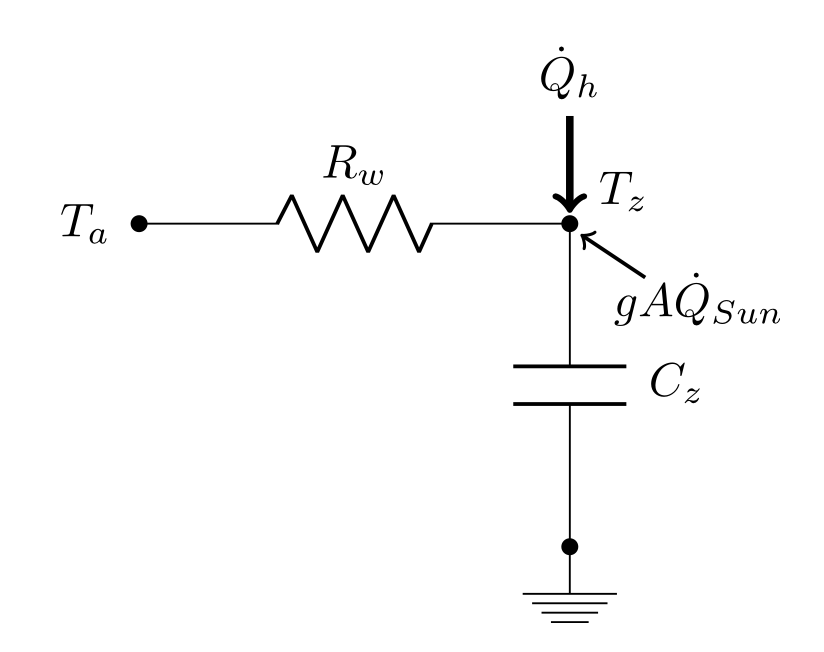
\includegraphics[scale=0.5]{images/single_zone.png}
\caption{RC Thermal network for a single zone lumped model.}
\label{fig:single_zone}
\end{figure}

Moreover, an additional heating source $\dot{Q_g}$ was introduced in order to account for the heat generated by the occupancy of the zone. Table \ref{tab:nomenclature_model} contains descriptions for all the above stated variables alongside their units.

\begin{table}[H]
\centering
\begin{tabular}{c|c|c}
Symbol & Variable & Units \\
\hline
\hline
$T_z$ & Zone average temperature & $K$\\
$T_a$ & Ambient temperature & $K$\\
$R_w$ & Wall thermal resistance & $K/W$\\
$C_z$ & Zone thermal capacitance & $J/K$\\
$gA$ & Window glazing factor $\cdot$ window area & $m^2$\\
$\dot{Q}_g$ & Heat input from occupancy & $W$\\
$\dot{Q}_{sun}$ & Heat input from solar radiation & $W/m^2$\\
$\dot{Q}_h$ & Heat input from radiator & $W$
\end{tabular}
\caption{Nomenclature for the proposed variables for the zone model.}
\label{tab:nomenclature_model}
\end{table}

In order to describe the thermal interactions for the thermal network,a derivation for an energy balance was done.

\begin{equation}
C_z \cdot \frac{d}{dt} T_z = \dot{Q}_h + gA \cdot \dot{Q}_{sun} + \dot{Q}_g + \frac{T_z(t)-T_a(t)}{R_w}
\label{eq:energy_balance}
\end{equation}

This equation allows for a full description of the temperature profile of the zone based on input data ($T_a, \dot{Q}_{sun}, \dot{Q}_g$ and $\dot{Q}_h$) and the zone constants ($R_w, C_z$ and $gA$). Weather data for the week of October 16 to 22, 2022 was acquired from \cite{nooa_2022} and the solar radiance accounting for cloud coverage for Belgium (specifically the Brussels area, Leuven included) was acquired from \cite{kunstmann} in order to achieve a realistic behavior for the zone temperature. A table containing this raw data is included in Appendix \ref{appendix}. Finally, the heating output due to occupancy was applied based off of the average heating output of a human adult (100W) and traditional working schedules (not at home during weekdays from 07:00-18:00). \\

Furthermore, the zone constants were tuned until a realistic behavior was achieved. These can be seen in Table \ref{tab:constants}. These constants are hereon assumed to be correct and will be the goal for the convergence of the trajectory optimization problem discussed in the following sections. Further explanation for this reverse-engineering approach is given in section \ref{sec:trajectory_optimization}.

\begin{table}[H]
\centering
\begin{tabular}{c|c}
Constant & Value\\
\hline
\hline
$C_z$ & 5000000 J/K\\
$R_w$ & 0.01 K/W\\
$gA$ & $0.45\cdot2.1$ m$^2$ 
\end{tabular}
\caption{Thermal zone constants.}
\label{tab:constants}
\end{table}

Once the data was gathered and the constants were determined, the behavior for the zone was modeled following a simple heating strategy on which the heating was turned on to maximum power whenever someone was home and turned completely off whenever someone was not. Figure \ref{fig:onoff_radiator} shows the resulting behavior for the zone temperature. Ideally, the zone temperature should be within the range of 20-25$^\circ$C (293.15-298.15K) to ensure thermal comfort for the users, pictured in the top subfigure in Figure \ref{fig:onoff_radiator} as the horizontal black lines. Finally, the running cost for the operation of the single radiator was calculated using the latest energy rate in Belgium (0.41 €/kWh) and is plotted for the entire week in the bottom subfigure of Figure \ref{fig:onoff_radiator}.\\

When analyzing Figure \ref{fig:onoff_radiator}, it is directly evident that the on/off strategy is not very effective economically and also in terms of thermal comfort. The temperature limits are crossed many times, reaching well over 300 K ($>27^\circ$C) on the weekend. Moreover, by opening the radiator to the maximum, plenty of energy gets wasted since, in many cases, the zone temperature is already within the thermal comfort limits and does not need further heating, just maintaining the temperature range. \\

With this in mind, an optimized strategy for the appropriate heat deployment for the entire week is developed with two different approaches in section \ref{sec:mpc} after the model identification in section \ref{sec:trajectory_optimization} is conducted.

\begin{figure}[H]
\centering
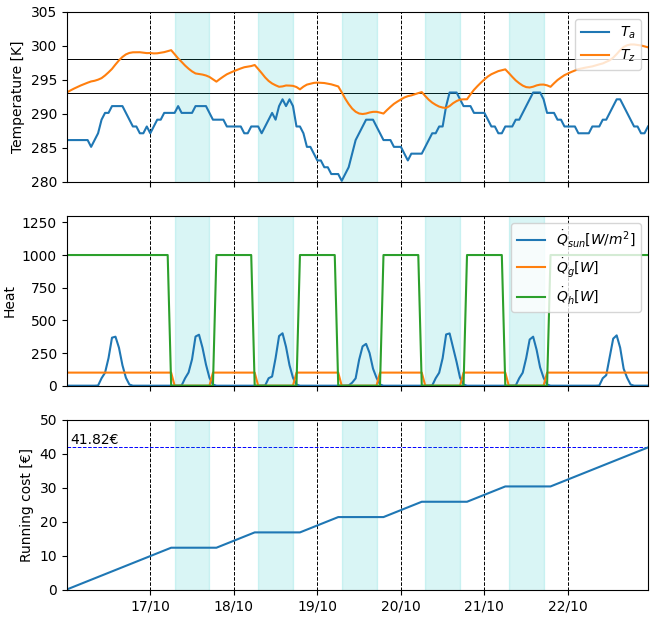
\includegraphics[scale=0.8]{images/onoff_radiator.png}
\caption{Zone temperature profile using a traditional on/off heating strategy.}
\label{fig:onoff_radiator}
\end{figure}
